%% Copernicus Publications Manuscript Preparation Template for LaTeX Submissions
%DIF LATEXDIFF DIFFERENCE FILE
%DIF DEL pre_response.tex    Tue Nov  7 08:55:30 2017
%DIF ADD post_response.tex   Tue Nov  7 13:00:14 2017
%% ---------------------------------
%% This template should be used for copernicus.cls
%% The class file and some style files are bundled in the Copernicus Latex Package, which can be downloaded from the different journal webpages.
%% For further assistance please contact Copernicus Publications at: production@copernicus.org
%% https://publications.copernicus.org/for_authors/manuscript_preparation.html


%% Please use the following documentclass and journal abbreviations for discussion papers and final revised papers.


%% 2-column papers and discussion papers
\documentclass[journal abbreviations, manuscript]{copernicus}



%% Journal abbreviations (please use the same for discussion papers and final revised papers)

% Archives Animal Breeding (aab)
% Atmospheric Chemistry and Physics (acp)
% Advances in Geosciences (adgeo)
% Advances in Statistical Climatology, Meteorology and Oceanography (ascmo)
% Annales Geophysicae (angeo)
% ASTRA Proceedings (ap)
% Atmospheric Measurement Techniques (amt)
% Advances in Radio Science (ars)
% Advances in Science and Research (asr)
% Biogeosciences (bg)
% Climate of the Past (cp)
% Drinking Water Engineering and Science (dwes)
% Earth System Dynamics (esd)
% Earth Surface Dynamics (esurf)
% Earth System Science Data (essd)
% Fossil Record (fr)
% Geographica Helvetica (gh)
% Geoscientific Instrumentation, Methods and Data Systems (gi)
% Geoscientific Model Development (gmd)
% Hydrology and Earth System Sciences (hess)
% History of Geo- and Space Sciences (hgss)
% Journal of Micropalaeontology (jm)
% Journal of Sensors and Sensor Systems (jsss)
% Mechanical Sciences (ms)
% Natural Hazards and Earth System Sciences (nhess)
% Nonlinear Processes in Geophysics (npg)
% Ocean Science (os)
% Proceedings of the International Association of Hydrological Sciences (piahs)
% Primate Biology (pb)
% Scientific Drilling (sd)
% SOIL (soil)
% Solid Earth (se)
% The Cryosphere (tc)
% Web Ecology (we)
% Wind Energy Science (wes)


%% \usepackage commands included in the copernicus.cls:
%\usepackage[german, english]{babel}
%\usepackage{tabularx}
%\usepackage{cancel}
%\usepackage{multirow}
%\usepackage{supertabular}
%\usepackage{algorithmic}
%\usepackage{algorithm}
%\usepackage{amsthm}
%\usepackage{float}
%\usepackage{subfig}
%\usepackage{rotating}
%DIF PREAMBLE EXTENSION ADDED BY LATEXDIFF
%DIF UNDERLINE PREAMBLE %DIF PREAMBLE
\RequirePackage[normalem]{ulem} %DIF PREAMBLE
\RequirePackage{color}\definecolor{RED}{rgb}{1,0,0}\definecolor{BLUE}{rgb}{0,0,1} %DIF PREAMBLE
\providecommand{\DIFadd}[1]{{\protect\color{blue}\uwave{#1}}} %DIF PREAMBLE
\providecommand{\DIFdel}[1]{{\protect\color{red}\sout{#1}}}                      %DIF PREAMBLE
%DIF SAFE PREAMBLE %DIF PREAMBLE
\providecommand{\DIFaddbegin}{} %DIF PREAMBLE
\providecommand{\DIFaddend}{} %DIF PREAMBLE
\providecommand{\DIFdelbegin}{} %DIF PREAMBLE
\providecommand{\DIFdelend}{} %DIF PREAMBLE
%DIF FLOATSAFE PREAMBLE %DIF PREAMBLE
\providecommand{\DIFaddFL}[1]{\DIFadd{#1}} %DIF PREAMBLE
\providecommand{\DIFdelFL}[1]{\DIFdel{#1}} %DIF PREAMBLE
\providecommand{\DIFaddbeginFL}{} %DIF PREAMBLE
\providecommand{\DIFaddendFL}{} %DIF PREAMBLE
\providecommand{\DIFdelbeginFL}{} %DIF PREAMBLE
\providecommand{\DIFdelendFL}{} %DIF PREAMBLE
%DIF END PREAMBLE EXTENSION ADDED BY LATEXDIFF

\begin{document}

\title{The National Eutrophication Survey: lake characteristics and historical nutrient concentrations}


% \Author[affil]{given_name}{surname}

\Author[1]{Joseph}{Stachelek}
\Author[2]{Chanse}{Ford}
\Author[3]{Dustin}{Kincaid}
\Author[1]{Katelyn}{King}
\Author[4]{Heather}{Miller}
\Author[5]{Ryan}{Nagelkirk}

\affil[1]{Department of Fisheries and Wildlife, Michigan State University, East Lansing, MI, USA}
\affil[2]{Department of Earth and Environmental Sciences, Michigan State University, East Lansing, MI, USA}
\affil[3]{Department of Integrative Biology, Michigan State University, East Lansing, MI, USA}
\affil[4]{Department of Microbiology and Molecular Genetics, Michigan State University, East Lansing, MI, USA}
\affil[5]{Department of Geography, Environment, and Spatial Sciences, Michigan State University, East Lansing, MI, USA}

%% The [] brackets identify the author with the corresponding affiliation. 1, 2, 3, etc. should be inserted.



\runningtitle{National Eutrophication Survey}

\runningauthor{Stachelek et al.}

\correspondence{Joseph Stachelek (stachel2@msu.edu)}



\received{}
\pubdiscuss{} %% only important for two-stage journals
\revised{}
\accepted{}
\published{}

%% These dates will be inserted by Copernicus Publications during the typesetting process.


\firstpage{1}

\maketitle



\begin{abstract}
Historical ecological surveys serve as a baseline and provide context for contemporary research, yet many of these records are not preserved in a way that ensures their long-term usability. The National Eutrophication Survey \DIFaddbegin \DIFadd{(NES) }\DIFaddend database is currently only available as scans of the original reports (PDF files) with no embedded character information. This limits its searchability, machine readability, and the ability of current and future scientists to systematically evaluate its contents. \DIFdelbegin \DIFdel{These }\DIFdelend \DIFaddbegin \DIFadd{The NES }\DIFaddend data were collected by the United States Environmental Protection Agency between 1972 and 1975 as part of an effort to investigate eutrophication in freshwater lakes and reservoirs. Although several studies have manually transcribed small portions of the database in support of specific studies, there have been no systematic attempts to transcribe and preserve the database in its entirety. Here we use a combination of automated optical character recognition and manual quality assurance procedures to make these data available for analysis. The performance of the optical character recognition protocol was found to be linked to variation in the quality (clarity) of the original documents. For each of the four archival scanned reports, our quality assurance protocol found an error rate between 5.9 and 17\%. The goal of our approach was to strike a balance between efficiency and data quality by combining hand-entry of data with digital transcription technologies. The finished database contains information on the physical characteristics, hydrology, and water quality of about 800 lakes in the contiguous United States (doi:10.5063/F10G3H3Z). Ultimately, this database could be combined with more recent studies to generate \DIFdelbegin \DIFdel{metadata analyses }\DIFdelend \DIFaddbegin \DIFadd{meta-analyses }\DIFaddend of water quality trends and spatial variation across the continental United States.
\end{abstract}


% \copyrightstatement{TEXT}


\introduction  %% \introduction[modified heading if necessary]
Effective management of inland freshwater lakes requires an understanding of the factors that affect water quality and how these factors change over time. One of these factors, termed eutrophication, occurs when excess nutrient inputs from human activities fuels increases in algal growth which can cause hypoxia and decreases in water clarity. Eutrophication of surface waters from increased phosphorus and nitrogen loading has been observed in connection with altered land-use especially in areas of rapid urbanization and intensive agriculture \citep{smith1999eutrophication, smith2014comment}. As human populations and their impacts continue to grow, eutrophication is expected to become more widespread \citep{bennett2001human, taranu2008quantifying}. Historical datasets are needed in order to track, understand, and manage eutrophication in lakes and reservoirs because they serve as an important baseline for modern studies. 

The U.S. Environmental Protection Agency (EPA) designed and implemented the National Eutrophication Survey (NES) in order to investigate the extent of eutrophication in freshwater lakes and reservoirs across the contiguous United States (US). Sampling took place in over 800 lakes and reservoirs from 1972 to 1975, and included a variety of physical, chemical, and biological metrics including data on nutrients and nutrient loading, hydrologic retention time, morphometry, and plankton community diversity. \DIFaddbegin \DIFadd{Each lake was sampled on a monthly basis for a period one year. Except for the phytoplankton distribution subset, which we did not transcribe \mbox{%DIFAUXCMD
\citep[see ][]{stomp2011large}}%DIFAUXCMD
, the NES data is provided as annual averages. }\DIFaddend Unlike current EPA National Lake Assessments that select a random sample of lakes across the US, the NES  targeted only lakes impacted directly or indirectly by municipal sewage treatment plant discharge \citep{nla-methods, nes-methods}. Until recently, these data were only available in their entirety as four separate scanned reports representing the northeastern and northcentral  (northeastern), eastern and southeastern (southeastern), central, and western regions of the US (Figure \ref{fig:points_regions}). In the remainder of the present paper we refer to the former two regions as simply the northeastern and southeastern regions.

\begin{figure*}[t]
  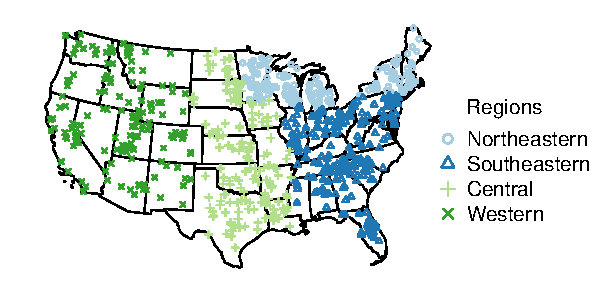
\includegraphics[width=12cm]{points_regions-crop.pdf}
  \caption{Survey locations colored by sampling year (1972 northeastern-red, 1973 southeastern-green, 1974 central-blue, 1975 western-grey).}\label{fig:points_regions}
\end{figure*}

To our knowledge, there have been no attempts to transcribe the data into a usable, searchable digital database despite its use in previous studies.   For example, large portions of the dataset were used to examine large scale relationships between residence time and phytoplankton abundance \citep{soballe1987large}. Also, it was used to predict eutrophication incidence in a Bayesian framework (Lamon and Stow 2004). Smaller portions of the data were used to explore drivers of nutrient loading \citep{stomp2011large,Brettreviewreassessmentlake2007}. Yet, to our knowledge, the only study to use the NES dataset and provide a publicly available data supplement is \citet{stomp2011large}, \DIFdelbegin \DIFdel{and }\DIFdelend \DIFaddbegin \DIFadd{but }\DIFaddend their data supplement was limited to a small subset of the available variables relating to phytoplankton community diversity. 

The present study is the first to leverage digital transcription technologies to unlock the full NES dataset. In this paper, we describe the digital transcription of the full NES dataset with the goal of making the dataset openly accessible to the research community. \DIFaddbegin \DIFadd{Specifically, our objective was to exactly reproduce the contents of the original dataset rather than to evaluate the its integrity. }\DIFaddend We introduce and publish the data in an open format that requires no proprietary software. It can be easily downloaded, used for analysis, and amended. The provided summary statistics and figures also allow users to quickly assess the utility of the data. \DIFdelbegin \DIFdel{. }\DIFdelend Finally, the code and raw data files are provided to facilitate the extraction of fields not represented in our completed dataset (mostly phytoplankton diversity data).

\section{Methods}

Data was collected from multiple locations within the water column and included in-situ measurements as well as laboratory \DIFdelbegin \DIFdel{analysis}\DIFdelend \DIFaddbegin \DIFadd{analyses}\DIFaddend . Flow estimates and drainage area calculations were provided by the USGS and were determined from flow gages when present. More detailed information on sampling methods, units, equipment, and accuracy can be found in the EPA survey methods publication \citep{nes-methods}. Due to historical nature of the dataset, the NES sampling design differs from more modern efforts \citep{nla-methods}. For example, the original NES data was collected from four separate regions of the US over the course of four years, whereas current assessments complete nation-wide sampling in a single summer. As such, NES data values represent the \DIFdelbegin \DIFdel{median }\DIFdelend \DIFaddbegin \DIFadd{mean }\DIFaddend of measurements taken in the spring, summer, and fall in either 1972 (northeastern), 1973 (southeastern), 1974 (central), or 1975 (western) rather than \DIFaddbegin \DIFadd{summer }\DIFaddend measurements taken in a single year.

We obtained the NES archival scanned reports from the EPA National Service Center for Environmental Publications (available at: https://www.epa.gov/nscep). The data for each NES region is contained in four separate files. We extracted the data from each file using automated techniques followed by manual quality assurance and checking \DIFaddbegin \DIFadd{of each value}\DIFaddend . To begin, we enhanced (de-noised) each file using the local adaptive filtering algorithm as provided by the Imagemagick program (v6.8.9-9, available at: https://www.imagemagick.org/). Next, we processed the enhanced files using the Tesseract optical character recognition program (OCR) \citep{R-tesseract, smith2007overview}. The output of these initial extraction steps were recorded in a set of “raw data” files where each file contains the raw unprocessed text of each document page. The contents of specific fields in the raw data were extracted to a database using the automated rules provided by the nesR software package \citep{R-nesR}. Finally, all values in the database were manually checked for accuracy against the original scanned reports. Inaccurate OCR outputs were hand-corrected in the final database. \DIFaddbegin \DIFadd{Because our goal was to reproduce the data from the original reports and not to verify the technical correctness of the original data, we only changed values if they did not match the orginal data reports. For example, we did not change data from the five NES lakes that had phosphate ($PO^4$) values exceeding their corresponding total phosphorus ($TP$) values despite the fact that this is not physically possible ($PO^4$ is a component of $TP$). 
}\DIFaddend 

We provide the final dataset in an open non-proprietary format (comma-delimited, *.csv). \DIFdelbegin \DIFdel{We }\DIFdelend \DIFaddbegin \DIFadd{In addition, we }\DIFaddend generated metadata descriptions from the contents of the original scanned reports. All calculations, table construction, and figure generation were performed in R and saved as reproducible R scripts \citep{R-core}. Table and figure generation was accomplished with the use of the reshape2, plyr, and sp packages \citep{R-plyr,R-sp}.

\section{Results}

The final NES dataset contains observations from 775 lakes and the distribution of these lakes was spatially variable. Although there were more lakes measured in the northeastern and southeastern United States, the number of locations was close to evenly distributed among the remaining regions (Figure \ref{fig:points_regions}, Table \ref{table:n}). Specifically, the number of lakes sampled in each region were as follows: northeastern - 200 lakes, southeastern - 245 lakes, central - 177 lakes, and western, 153 lakes. 

\begin{table*}
\caption{Number of measurements (n) for each variable in each NES region.}\label{table:n}
\begin{tabular}{lllll}
\tophline
Variable & Western & Central & Northeastern & Southeastern\\
\middlehline
Drainage area & 122 & 138 & 171 & 232\\
\DIFdelbeginFL %DIFDELCMD < \hline
%DIFDELCMD < %%%
\DIFdelendFL \DIFaddbeginFL 

\DIFaddendFL Surface area & 152 & 177 & 200 & 245\\

Mean depth & 149 & 174 & 174 & 242\\

Total inflow & 124 & 138 & 170 & 232\\

Retention time & 124 & 140 & 158 & 230\\

Alkalinity & 153 & 177 & 200 & 245\\

Conductivity & 153 & 176 & 200 & 245\\

Secchi depth & 153 & 177 & 200 & 245\\

Total P & 153 & 177 & 200 & 245\\

Total inorg. P & 153 & 177 & 200 & 245\\

Total inorg. N & 153 & 177 & 200 & 245\\

Total N & 152 & 176 & 1 & 245\\

P pt. source mun. & 52 & 83 & 139 & 189\\

P pt. source ind. & 7 & 1 & 10 & 24\\

P pt. source sep. & 65 & 88 & 111 & 175\\

P nonpt. source & 122 & 133 & 167 & 231\\

P total inputs & 122 & 133 & 167 & 231\\

N pt. source mun. & 52 & 84 & 139 & 189\\

N pt. source ind. & 7 & 1 & 8 & 22\\

N pt. source sep. & 77 & 90 & 111 & 184\\

N nonpt. source & 122 & 129 & 167 & 231\\

N total inputs & 122 & 129 & 167 & 231\\

P total exports & 119 & 132 & 167 & 227\\

P retention & 99 & 115 & 144 & 201\\

P load per area & 122 & 133 & 167 & 231\\

N total exports & 119 & 133 & 166 & 227\\

N retention & 88 & 111 & 122 & 170\\

N load per area & 122 & 135 & 167 & 231\\
\bottomhline
\end{tabular}
\end{table*}

%DIF < \begin{table*}[t]
%DIF < \caption{TEXT}
%DIF < \begin{tabular}{column = lcr}
%DIF < \tophline
%DIF < 
%DIF < \middlehline
%DIF < 
%DIF < \bottomhline
%DIF < \end{tabular}
%DIF < \belowtable{} % Table Footnotes
%DIF < \end{table*}
\DIFdelbegin %DIFDELCMD < 

%DIFDELCMD < %%%
\DIFdel{Although the overall }\DIFdelend \DIFaddbegin \DIFadd{In addition to differences in the total }\DIFaddend number of lakes \DIFdelbegin \DIFdel{was similar among regions, they differed }\DIFdelend \DIFaddbegin \DIFadd{measured in each region, there were also differences }\DIFaddend in the proportion of lakes classified as impoundments rather than \DIFaddbegin \DIFadd{as }\DIFaddend natural lakes. For example, slightly more than half of \DIFaddbegin \DIFadd{all }\DIFaddend the lakes studied (462 of 775) were classified as impoundments yet the northeastern region had only 54 impoundments \DIFdelbegin \DIFdel{and }\DIFdelend \DIFaddbegin \DIFadd{while }\DIFaddend the southeastern region had 168 impoundments. Conversely, the number of natural lakes sampled in the northeastern region (146 lakes) was more than double that of any other region (77, 48, and 42, for southeastern, western, and central United States, respectively).

We observed substantial spatial variation in many of the individual lake characteristics. For example, lakes in the eastern sub-regions were generally smaller and shallower than lakes in the western sub-region (Table \ref{table:means}). In addition, lakes in the western sub-region generally had higher alkalinity and higher water clarity (Figure \ref{fig:alkalinity}, \ref{fig:secchi}). Lakes with particularly low alkalinity were found in coastal areas, whereas lakes with particularly high alkalinity were found in Nevada, western Washington, and parts of North Dakota. Comparisons among regions was easy for some well-sampled lake chemistry parameters such as total phosphorus but more difficult for undersampled lake chemistry parameters. A particularly extreme example of this difficulty was total nitrogen measurements in the eastern region, as this parameter was only measured for a single lake (Table \ref{table:n}). 

\begin{table*}[t]
\caption{Mean and standard deviation (sd) for each variable in each NES region.}\label{table:means}
\begin{tabular}{lllllllllllll}
\tophline
\DIFdelbeginFL %DIFDELCMD < \multicolumn{1}{l|}{Region} %%%
\DIFdelendFL \DIFaddbeginFL \multicolumn{1}{l}{Region} \DIFaddendFL & \DIFdelbeginFL %DIFDELCMD < \multicolumn{3}{|c|}{Western} %%%
\DIFdelendFL \DIFaddbeginFL \multicolumn{3}{c}{Western} \DIFaddendFL & \DIFdelbeginFL %DIFDELCMD < \multicolumn{3}{|c|}{Central} %%%
\DIFdelendFL \DIFaddbeginFL \multicolumn{3}{c}{Central} \DIFaddendFL & \DIFdelbeginFL %DIFDELCMD < \multicolumn{3}{|c|}{Northeastern} %%%
\DIFdelendFL \DIFaddbeginFL \multicolumn{3}{c}{Northeastern} \DIFaddendFL & \DIFdelbeginFL %DIFDELCMD < \multicolumn{3}{|c}{Southeastern} %%%
\DIFdelendFL \DIFaddbeginFL \multicolumn{3}{c}{Southeastern} \DIFaddendFL \\ \cline{1-1} \cline{2-4} \cline{5-7} \cline{8-10} \cline{11-13}
Variable & Mean &   & sd & Mean &   & sd & Mean &   & sd & Mean &   & sd\\
\middlehline
Drainage area ($km^{2}$) & 2.5e+04 & ± & 7.8e+04 & 2.1e+04 & ± & 7.5e+04 & 3.2e+03 & ± & 1.4e+04 & 5.3e+03 & ± & 1.4e+04\\

Surface area ($km^{2}$) & 44.57 & ± & 99.83 & 54.38 & ± & 1.4e+02 & 27.25 & ± & 99.01 & 42.7 & ± & 1.4e+02\\

Mean depth ($m$) & 16.71 & ± & 27.08 & 5.97 & ± & 4.49 & 7 & ± & 9.37 & 6.4 & ± & 6.07\\

Total inflow ($m^{3} \cdot s^{-1}$) & 52.1 & ± & 1.1e+02 & 31.82 & ± & 71.77 & 23.1 & ± & 65.26 & 82.6 & ± & 2.3e+02\\

Retention time ($years$) & 7.27 & ± & 43.32 & 2.78 & ± & 6.98 & 2.01 & ± & 4.77 & 0.59 & ± & 1.12\\

Alkalinity ($mg \cdot l^{-1}$) & 1.7e+02 & ± & 3.7e+02 & 1.5e+02 & ± & 91.51 & 1.2e+02 & ± & 1.6e+02 & 72.18 & ± & 66.25\\

Conductivity ($uohm$) & 4.9e+02 & ± & 1.0e+03 & 6.4e+02 & ± & 7.6e+02 & 3.3e+02 & ± & 4.0e+02 & 2.5e+02 & ± & 2.2e+02\\

Secchi depth ($m$) & 2.86 & ± & 2.64 & 1.2 & ± & 0.91 & 1.81 & ± & 1.71 & 1.22 & ± & 0.82\\

Total P ($mg \cdot l^{-1}$) & 0.07 & ± & 0.13 & 0.11 & ± & 0.16 & 0.16 & ± & 0.35 & 0.12 & ± & 0.27\\

Total inorg. P ($mg \cdot l^{-1}$) & 0.04 & ± & 0.11 & 0.04 & ± & 0.07 & 0.11 & ± & 0.3 & 0.05 & ± & 0.15\\

Total inorg. N ($mg \cdot l^{-1}$) & 0.14 & ± & 0.23 & 0.33 & ± & 0.58 & 0.47 & ± & 0.66 & 0.72 & ± & 0.91\\

Total N ($mg \cdot l^{-1}$) & 0.62 & ± & 0.65 & 1.22 & ± & 1.11 & 0.12 & ± & NA & 1.56 & ± & 1.25\\

P pt. source mun. ($kg \cdot yr^{-1}$) & 2.5e+04 & ± & 8.7e+04 & 2.3e+04 & ± & 5.6e+04 & 3.5e+04 & ± & 1.5e+05 & 4.5e+04 & ± & 1.1e+05\\

P pt. source ind. ($kg \cdot yr^{-1}$) & 2.5e+04 & ± & 4.0e+04 & 1.3e+04 & ± & NA & 2.7e+04 & ± & 4.9e+04 & 1.7e+04 & ± & 4.5e+04\\

P pt. source sep. ($kg \cdot yr^{-1}$) & 56.62 & ± & 1.4e+02 & 60.62 & ± & 93.67 & 1.6e+02 & ± & 3.4e+02 & 98.55 & ± & 2.3e+02\\

P nonpt. source ($kg \cdot yr^{-1}$) & 1.4e+05 & ± & 4.2e+05 & 1.8e+05 & ± & 6.8e+05 & 5.6e+04 & ± & 2.1e+05 & 1.9e+05 & ± & 5.5e+05\\

P total inputs ($kg \cdot yr^{-1}$) & 1.5e+05 & ± & 4.7e+05 & 2.0e+05 & ± & 7.0e+05 & 8.7e+04 & ± & 3.4e+05 & 2.3e+05 & ± & 5.8e+05\\

N pt. source mun. ($kg \cdot yr^{-1}$) & 7.8e+04 & ± & 2.5e+05 & 7.3e+04 & ± & 1.7e+05 & 1.4e+05 & ± & 5.4e+05 & 1.4e+05 & ± & 3.8e+05\\

N pt. source ind. ($kg \cdot yr^{-1}$) & 2.3e+07 & ± & 6.1e+07 & 4.0e+03 & ± & NA & 1.6e+05 & ± & 4.2e+05 & 1.7e+05 & ± & 5.6e+05\\

N pt. source sep. ($kg \cdot yr^{-1}$) & 5.7e+06 & ± & 5.0e+07 & 2.2e+03 & ± & 3.5e+03 & 4.3e+03 & ± & 5.5e+03 & 3.3e+03 & ± & 6.7e+03\\

N nonpt. source ($kg \cdot yr^{-1}$) & 1.8e+06 & ± & 4.9e+06 & 1.8e+06 & ± & 4.4e+06 & 1.2e+06 & ± & 4.1e+06 & 3.1e+06 & ± & 8.9e+06\\

N total inputs ($kg \cdot yr^{-1}$) & 6.8e+06 & ± & 5.7e+07 & 1.8e+06 & ± & 4.3e+06 & 1.3e+06 & ± & 4.6e+06 & 3.2e+06 & ± & 9.0e+06\\

P total exports ($kg \cdot yr^{-1}$) & 6.2e+04 & ± & 1.7e+05 & 7.4e+04 & ± & 1.9e+05 & 7.3e+04 & ± & 3.1e+05 & 1.9e+05 & ± & 6.3e+05\\

P retention (\%) & 47.77 & ± & 28.5 & 57.55 & ± & 26.01 & 36.93 & ± & 25.2 & 42.7 & ± & 23.34\\

P load per area($g / m^{2} / day$) & 5.61 & ± & 21.36 & 3.3 & ± & 9.2 & 28.46 & ± & 97.49 & 9.43 & ± & 17.06\\

N total exports ($kg \cdot yr^{-1}$) & 1.6e+06 & ± & 4.0e+06 & 1.2e+06 & ± & 2.8e+06 & 1.2e+06 & ± & 4.9e+06 & 3.0e+06 & ± & 8.3e+06\\

N retention (\%) & 39.33 & ± & 27.13 & 43.41 & ± & 23.97 & 28.41 & ± & 23.62 & 26.28 & ± & 18.85\\

N load per area ($g / m^{2} / day$) & 1.8e+02 & ± & 1.1e+03 & 42.67 & ± & 1.1e+02 & 2.8e+02 & ± & 9.1e+02 & 1.3e+02 & ± & 2.4e+02\\
\bottomhline
\end{tabular}
\end{table*}

\begin{figure*}[t]
  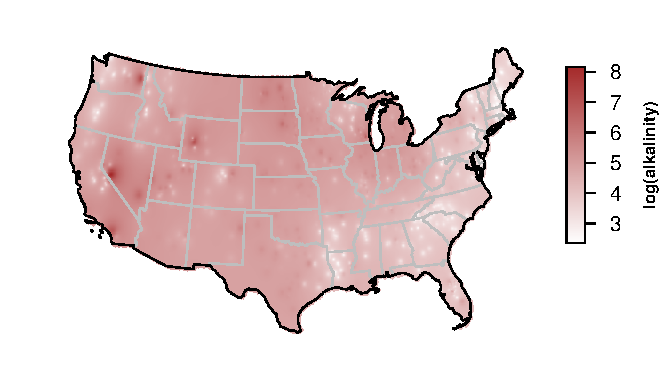
\includegraphics[width=12cm]{alkalinity-crop.pdf}
  \caption{Map of log-scaled alkalinity (mg/L) interpolated using inverse distance weighting.}\label{fig:alkalinity}
\end{figure*}

\begin{figure*}[t]
  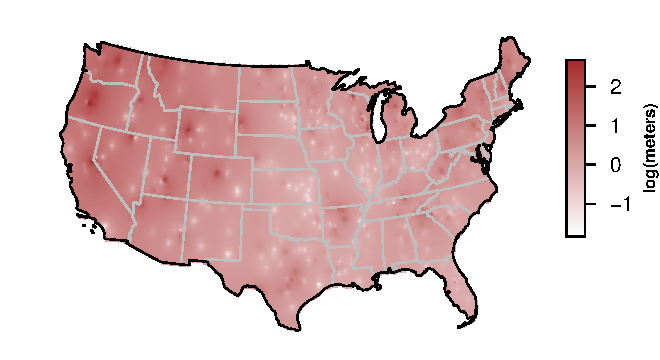
\includegraphics[width=12cm]{secchi-crop.pdf}
  \caption{Map of secchi depth (m) interpolated using inverse distance weighting.}\label{fig:secchi}
\end{figure*}

The ability to examine these spatial trends was made possible by our optical character recognition procedure which had 6 - 17\% accuracy depending on region and archival report scan quality. In total, we carried out approximately 5,000 hand-corrections to the automated data product as part of our manual quality control review. A total of approximately 650 lakes had values for at least 80\% of the total number of variables shown in Table \ref{table:n}. On an individual lake basis, the most common “missing” data was nutrient loading estimates for individual point and nonpoint-source components. In many cases, this data may not actually be missing but it may have not been a component of the budget for that particular lake. For example, not all lakes have industrial land use so no data is expected in these cases.

\section{Discussion}

We have demonstrated an approach for rescuing historical data from scanned documents. In particular, our approach involved a two-step process of automated data scraping followed by hand-curation and quality assurance. Overall, we found that optical character recognition was an efficient method for reducing the labor associated with transcribing analog text records \citep{drinkwater2014use}. Unfortunately, optical character recognition technology does not have absolute accuracy. In our case, transcription was hampered by poor print and scan quality of the source paper documents. We discovered through our manual validation procedure that the OCR computations produced inaccurate values in approximately 6 - 17\% of the cells in the complete dataset (n = 4836). We expect that accuracy could be improved by experimenting with varying the window size of the local adaptive thresholding algorithm relative to the document font size. Our ability to experiment with thresholding window size was limited due to the computationally expensive nature of these extractions.

The end result of our approach was data from every lake and nearly every variable in the NES survey dataset. The only primary subset of the NES data which is not included in our final product is the phytoplankton distribution data which has already been digitally transcribed by \citet{stomp2011large}. The results of the present study could be used to explore anthropogenic and environmental drivers of lake eutrophication as well as to verify previously documented trends. One example is the 2007 National Lakes Assessment (NLA) Report, which included a reanalysis of some of the NES study lakes \citep{nla-methods}. This reanalysis considered population level trends in the NES lakes but did not consider trends in individual lakes or potential environmental drivers contributing to observed trends. On a population basis, the NLA reanalysis found that less than 30\% of the NES lakes had increased chlorophyll and phosphorus concentrations. The results of the present study could be used to verify these claims as well as to compare the NES data with more recent work such as the 2012 National Lakes Assessment.  Note that sampling techniques may differ from current techniques, so care should be given when making comparisons. In addition to their utility in validating historical trends, this dataset has value because it contains data on a number of hydrographic variables which are difficult to estimate such as water residence (retention) time. Such data is critical to a variety of hydrological and water quality modelling efforts \citep{Brettreviewreassessmentlake2007}. 

Although our goal was to digitally transcribe the full NES dataset to facilitate studies on historical nutrient loading, it is worth noting the similarities between the present study and other scientific record digitization initiatives. Such initiatives are common in the climate and ocean sciences but they are just starting to gain momentum in the biological sciences \citep{allan2011international, freeman2017icoads}. To our knowledge, the present study is the first large-scale attempt at digitization of historical limnology records. We hope that by making our analysis open and reproducible we will inspire future efforts at recovering important records from the pre-digital era.

%% The following commands are for the statements about the availability of data sets and/or software code corresponding to the manuscript.
%% It is strongly recommended to make use of these sections in case data sets and/or software code have been part of your research the article is based on.

% \codeavailability{TEXT} %% use this section when having only software code available

% \dataavailability{} %% use this section when having only data sets available

\codedataavailability{
Original scanned reports from the EPA are available from the EPA National Service Center for Environmental Publications (https://www.epa.gov/nscep).  Our cleaned and useable data are available for download at doi:10.5063/F10G3H3Z. The data are provided as a zip file which contains all versions of the data including the raw and quality checked versions \citep{nes}. Moreover, the R package and R code used to scrape and analyze the data are provided by \citet{R-nesR} so that the methods may be reproduced and openly available for (re)use. All figures and summary statistics were generated by R scripts available in the data supplement linked above.
} %% use this section when having data sets and software code available

% \appendix
% \section{}    %% Appendix A
% 
% \subsection{}     %% Appendix A1, A2, etc.


% \noappendix       %% use this to mark the end of the appendix section

%% Regarding figures and tables in appendices, the following two options are possible depending on your general handling of figures and tables in the manuscript environment:

%% Option 1: If you sorted all figures and tables into the sections of the text, please also sort the appendix figures and appendix tables into the respective appendix sections.
%% They will be correctly named automatically.

%% Option 2: If you put all figures after the reference list, please insert appendix tables and figures after the normal tables and figures.
%% To rename them correctly to A1, A2, etc., please add the following commands in front of them:

\appendixfigures  %% needs to be added in front of appendix figures

\appendixtables   %% needs to be added in front of appendix tables

%% Please add \clearpage between each table and/or figure. Further guidelines on figures and tables can be found below.



\authorcontribution{
All authors contributed to data quality assurance and edited the article text. JS conceived the study and implemented the optical character recognition code. CF, DK, and RN performed the data analysis and made figures. KK, HM, and JS wrote major parts of the manuscript text.
} %% optional section

\competinginterests{
The authors declare that they have no conflict of interest.
} %% this section is mandatory even if you declare that no competing interests are present

% \disclaimer{TEXT} %% optional section

% \begin{acknowledgements}
% TEXT
% \end{acknowledgements}


%% REFERENCES

%% The reference list is compiled as follows:

% \begin{thebibliography}{}
% 
% \bibitem[AUTHOR(YEAR)]{LABEL}
% REFERENCE 1
% 
% \bibitem[AUTHOR(YEAR)]{LABEL}
% REFERENCE 2
% 
% \end{thebibliography}

%% Since the Copernicus LaTeX package includes the BibTeX style file copernicus.bst,
%% authors experienced with BibTeX only have to include the following two lines:
%%
\bibliographystyle{copernicus}
\bibliography{bib.bib}
%%
%% URLs and DOIs can be entered in your BibTeX file as:
%%
%% URL = {http://www.xyz.org/~jones/idx_g.htm}
%% DOI = {10.5194/xyz}


%% LITERATURE CITATIONS
%%
%% command                        & example result
%% \citet{jones90}|               & Jones et al. (1990)
%% \citep{jones90}|               & (Jones et al., 1990)
%% \citep{jones90,jones93}|       & (Jones et al., 1990, 1993)
%% \citep[p.~32]{jones90}|        & (Jones et al., 1990, p.~32)
%% \citep[e.g.,][]{jones90}|      & (e.g., Jones et al., 1990)
%% \citep[e.g.,][p.~32]{jones90}| & (e.g., Jones et al., 1990, p.~32)
%% \citeauthor{jones90}|          & Jones et al.
%% \citeyear{jones90}|            & 1990



%% FIGURES

%% When figures and tables are placed at the end of the MS (article in one-column style), please add \clearpage
%% between bibliography and first table and/or figure as well as between each table and/or figure.


%% ONE-COLUMN FIGURES

%%f
%\begin{figure}[t]
%\includegraphics[width=8.3cm]{FILE NAME}
%\caption{TEXT}
%\end{figure}
%
%%% TWO-COLUMN FIGURES
%
%%f
%\begin{figure*}[t]
%\includegraphics[width=12cm]{FILE NAME}
%\caption{TEXT}
%\end{figure*}
%
%
%%% TABLES
%%%
%%% The different columns must be seperated with a & command and should
%%% end with \\ to identify the column brake.
%
%%% ONE-COLUMN TABLE
%
%%t
%\begin{table}[t]
%\caption{TEXT}
%\begin{tabular}{column = lcr}
%\tophline
%
%\middlehline
%
%\bottomhline
%\end{tabular}
%\belowtable{} % Table Footnotes
%\end{table}
%
%%% TWO-COLUMN TABLE
%
%%t
%\begin{table*}[t]
%\caption{TEXT}
%\begin{tabular}{column = lcr}
%\tophline
%
%\middlehline
%
%\bottomhline
%\end{tabular}
%\belowtable{} % Table Footnotes
%\end{table*}
%
%
%%% MATHEMATICAL EXPRESSIONS
%
%%% All papers typeset by Copernicus Publications follow the math typesetting regulations
%%% given by the IUPAC Green Book (IUPAC: Quantities, Units and Symbols in Physical Chemistry,
%%% 2nd Edn., Blackwell Science, available at: http://old.iupac.org/publications/books/gbook/green_book_2ed.pdf, 1993).
%%%
%%% Physical quantities/variables are typeset in italic font (t for time, T for Temperature)
%%% Indices which are not defined are typeset in italic font (x, y, z, a, b, c)
%%% Items/objects which are defined are typeset in roman font (Car A, Car B)
%%% Descriptions/specifications which are defined by itself are typeset in roman font (abs, rel, ref, tot, net, ice)
%%% Abbreviations from 2 letters are typeset in roman font (RH, LAI)
%%% Vectors are identified in bold italic font using \vec{x}
%%% Matrices are identified in bold roman font
%%% Multiplication signs are typeset using the LaTeX commands \times (for vector products, grids, and exponential notations) or \cdot
%%% The character * should not be applied as mutliplication sign
%
%
%%% EQUATIONS
%
%%% Single-row equation
%
%\begin{equation}
%
%\end{equation}
%
%%% Multiline equation
%
%\begin{align}
%& 3 + 5 = 8\\
%& 3 + 5 = 8\\
%& 3 + 5 = 8
%\end{align}
%
%
%%% MATRICES
%
%\begin{matrix}
%x & y & z\\
%x & y & z\\
%x & y & z\\
%\end{matrix}
%
%
%%% ALGORITHM
%
%\begin{algorithm}
%\caption{?}
%\label{a1}
%\begin{algorithmic}
%?
%\end{algorithmic}
%\end{algorithm}
%
%
%%% CHEMICAL FORMULAS AND REACTIONS
%
%%% For formulas embedded in the text, please use \chem{}
%
%%% The reaction environment creates labels including the letter R, i.e. (R1), (R2), etc.
%
%\begin{reaction}
%%% \rightarrow should be used for normal (one-way) chemical reactions
%%% \rightleftharpoons should be used for equilibria
%%% \leftrightarrow should be used for resonance structures
%\end{reaction}
%
%
%%% PHYSICAL UNITS
%%%
%%% Please use \unit{} and apply the exponential notation


\end{document}
